%%%%%%%%%%%%%%%%%%%%%%%%%%%%%%%%%%%%%%%%%%%%%%%%%%%%%%%%%%%%%%%%%%%%%%%%%%
\chapter{Analýza bajtkódu}\label{Analysis}

% Popis způsobu analýzy rozsáhlého vzorku testovacích dat, prezentace výsledků a zhodnocení.

V~této kapitole popisuji výsledky analýzy bajtkódu. Pomocí nástroje \texttt{jbyco} jsem získala data reprezentující vybraný vzorek testovacích souborů a tato data následně zpracovala a vyhodnotila. Zkoumala jsem velikosti položek v~\texttt{class} souborech, využití lokálních proměnných a parametrů metod a typické sekvence instrukcí.

Testovací vzorek jsem vytvořila z~\texttt{jar} souborů stažených z~\texttt{http://mvnrepository.com}. Z~populárních kategorií jsem vybrala nejčastěji stahované soubory. Pracovala jsem se dvěmi testovacími vzorky. Velký vzorek se skládal z 95 souborů o celkové velikosti 102,4 MB a obsahoval 59 229 \texttt{class} souborů. Menší vzorek se skládal z 80 souborů o velikosti 46,6 MB a obsahoval 27 981
\texttt{class} souborů. Menší vzorek jsem použila pro vyhledání typických sekvencí instrukcí.

\section{Výsledky analýzy}\label{AnalysisResults}

Typický \texttt{class} soubor z velkého vzorku obsahuje v průměru 117 konstant v tabulce konstant, 2 členské proměnné, 8 metod, 163 instrukcí a 29 atributů. Ze zkoumání celkové velikosti těchto položek vyplynulo, že 64\% z celkové velikosti všech souborů tvoří konstanty, 0,7\% členské proměnné bez konstant, 2,1\% metody bez konstant a atributů a 10\% instrukce.

Při bližším pohledu na velikosti konstant se ukázalo, že 57\% z celkové velikosti souborů tvoří pouze konstanty typu \textit{constant\_utf8}. Tedy konstanty popisující řetězce. Velikosti ostatních konstant jsou zanedbatelné. Řetězce popisující názvy a typy tříd, metod a členských proměnných tvoří 61\% z celkové velikosti konstant typu \textit{constant\_utf8}.

Součet velikostí všech atributů ku celkové velikosti souborů tvoří 47\%, ale tato hodnota je nepřesná, neboť atributy mohou být součástí jiných atributů a jejich velikost je tedy započítána vícekrát. Nejvýznamnější z hlediska velikosti jsou atribut \texttt{Code} s velikostí 30\% z celkové velikosti souborů a součet velikostí informativních atributů s velikostí 14\%.

Zkoumání instrukcí z hlediska jejich velikosti ukázalo, že prvních pět nejobjemnějších instrukcí tvoří 40\% z celkové velikosti instrukcí. Jsou to instrukce pro volání metod, načtení hodnoty z členské proměnné a načtení reference na objekt z lokální proměnné s indexem 0. Na této pozici se často vyskytuje reference na aktuální objekt. Z instrukcí s proměnnou délkou má instrukce \texttt{tableswitch} v průměru velikost 107 B a instrukce \texttt{lookupswitch} velikost 43 B.

% TODO tabulka celkových velikostí
% TODO tabulka řetězců
% TODO tabulka informativních atributů
% TODO tabulka nejčastějších instrukcí

Data popisující využití parametrů a lokálních proměnných jsou znázorněna v grafech \ref{params} a \ref{vars}. Z dat vyplývá, že z lokálních proměnných obsahujících argumenty metody se tyto hodnoty načtou průměrně jedenkrát a dále se s nimi nepracuje. S nižším indexem proměnné počet načítání roste až k hodnotě 2,544 pro index 0. V tomto indexu se u nestatických metod předává reference na aktuální objekt (\texttt{this}). S lokálními proměnnými, které neslouží k předávání parametrů, se průměrně provádí 4,18 operací načítání, 1,76 operací vkládání a 0,25 operací inkrementace.

\begin{figure}[h!]
\centering
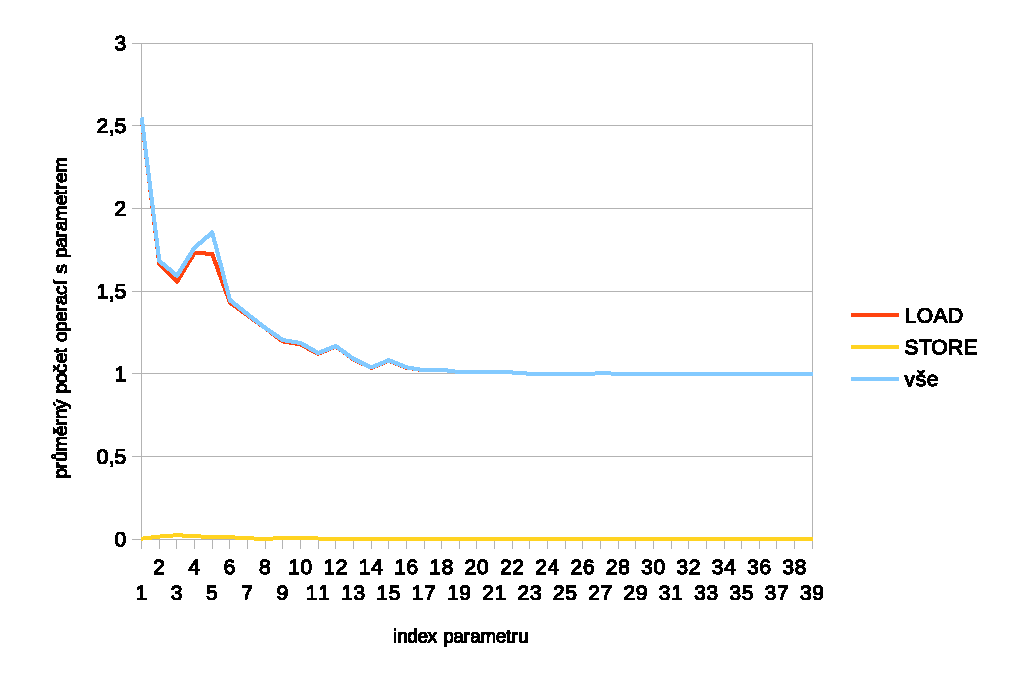
\includegraphics[scale=0.9]{fig/params}
\caption{Průměrné počty operací s parametry metod.}\label{params}
\end{figure}

\begin{figure}[h!]
\centering
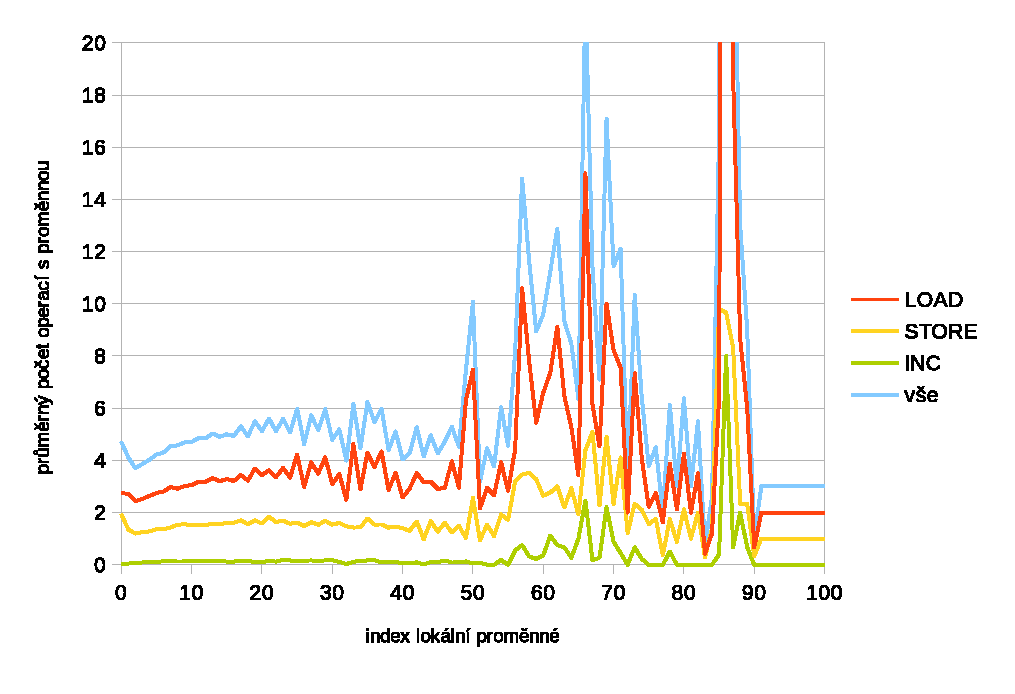
\includegraphics[scale=0.9]{fig/locals} 
\caption{Průměrné počty operací s lokálními proměnnými.}\label{vars}
\end{figure}

\section{Vyhodnocení}\label{AnalysisSummary}
